% Explicar en que consitió el trabajo (brevemente).
	% - Explicar levemente los criterios usados para la paralelización
	% - Por qué es buena idea usar este tipo de procesamiento en filtros de imágenes. (todos los pixeles reciben exactamente el mismo procesamiento y así en una sola ráfaga se peude levantar y procesar muchos).
	% - Explicar la hipótesis (debería ser n veces mas rápido porque zarasa).
	% - Se intentó estudiar si vale la pena o no el esfuerzo adicional de desarrollo y debuggeo.


Para analizar el modelo de procesamiento SIMD se implementaron tres filtros; dos de video\footnote{Los filtros de video implementados son técnicamente filtros de imágenes aplicados a los múltiples cuadros de un video.} y uno de imágenes. Para cada uno de ellos se desarrollaron implementaciones tanto en lenguaje C como en lenguaje ensamblador, utilizando la familia de extensiones SSE (\textbf{S}treaming \textbf{S}IMD \textbf{E}xtensions) de la arquitectura Intel.

Sobre las implementaciones logradas, se estudiaron las diferencias en eficiencia y en costo de desarrollo entre las soluciones en C o en ASM, así como el costo temporal relativo entre las diferentes partes de cada solución. Por ejemplo, se analizó el impacto de los saltos condicionales en una implementación en C o la relación entre tiempo de lectura/escritura, procesamiento y lógica de flujo en un programa en lenguaje ensamblador.

Posteriormente, se compararon las características y la eficiencia de los distintos niveles de optimización provistos por compiladores típicos, así como el beneficio de incorporar variadas estrategias algorítmicas de optimización sobre las implementaciones en lenguaje ensamblador, como la técnica de desenrollado de ciclos en un filtro de video o la técnica de entubado de código en el filtro de imágenes.

Cada una de las experiencias con los tres filtros desarrollados se describen en detalle y por separado en secciones subsiguientes.

\subsection{Modelo de procesamiento SIMD}

El procesamiento SIMD consiste en realizar una misma operación sobre una gran cantidad de datos de manera simultánea y atómica, logrando lo que se conoce como paralelismo a nivel de datos. Los filtros de imágenes y otros procesos sobre multimedia son particularmente propicios para este tipo de procesamiento ya que habitualmente requieren realizar un mismo tipo de cálculo sobre cientos o miles de puntos, por lo cual la posibilidad de trabajar en bloque provee un claro beneficio en tiempo de ejecución en comparación a un procesamiento en serie.

\begin{figure}[h]
\begin{center}
  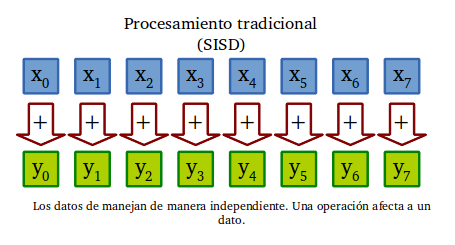
\includegraphics[scale=0.4]{secciones/introduccion/imagenes/SISD.png}
    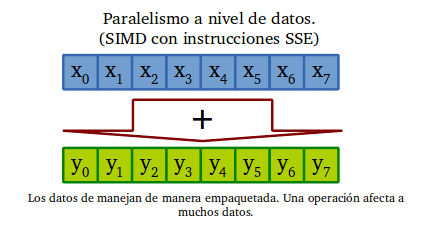
\includegraphics[scale=0.4]{secciones/introduccion/imagenes/SIMD.png}
\end{center}
\caption{Esquemas de procesamiento SISD y SIMD}
\label{fig:SISD-SIMD}
\end{figure}

La figura \ref{fig:SISD-SIMD} compara el esquema SIMD con un tipo de procesamiento más tradicional, donde para realizar una serie de sumas es necesario realizarlas independientemente y en múltiples pasos. Bajo el modelo SIMD, los datos se manejan de forma empaquetada y las sumas se realizan en simultáneo y con un costo que es idealmente independiente de la cantidad de datos.

La intuición parecería indicar que a priori se debería esperar un beneficio en eficiencia proporcional a la multiplicidad de datos que se manipulan en simultáneo. Es decir, al procesar 4 datos a la vez se esperaría obtener un proceso 4 veces más rápido, al procesar 8 datos a la vez uno 8 veces más rápido, etc. Sin embargo, la experiencia muestra que la relación entre ambas magnitudes es compleja, por lo cual es relevante contemplar diferentes factores característicos de la arquitectura Intel como la velocidad de acceso a memoria o el uso de la caché, así como el medio en el cuál se realiza la experimentación, y los algoritmos utilizados.

% (esto quedo mas o menos dicho arriba y dicho varias veces más adelante)
% 	A lo largo del trabajo se va a ir mostrando como el uso de código de ensamblador
% optimizado para el uso de la tecnología SSE produce programas sumamente eficientes. Sin embargo
% producir ese código es sumamente trabajoso, mucho mas que usar lenguajes de mas alto nivel como
% c o c++. Por ese motivo se intentará hacer otro análisis (tal vez algo menos científico
% pero intentando justificar de la manera mas objetiva posible) de cuando vale la pena y cuando no.

Naturalmente, existen procesos cuyas características imponen limitaciones a la aplicación de este esquema de procesamiento. En muchos casos el motivo de estas limitaciones consiste en una dependencia de datos entre diferentes partes del algorítmo, o una distribución irregular entre los datos que se precisa leer o escribir, inhibiendo el procesamiento en bloque. Tal es el caso de una rotación de ángulo arbitrario, donde datos consecutivos en la entrada no ocupan posiciones consecutivas en la salida.